%!TEX root = guided_inpainting_paper.tex
\section{Introduction}
Image inpainting is the task to fill in the missing part of an image with visually plausible contents. It is one of the most common operations of image editing~\cite{gatys2015texture} and low-level computer visions~\cite{komodakis2006image,hays2007scene}. The goal of image inpainting is to create semantically plausible contents with realistic texture details. The inpainting can either be consistent with the original image or be different but coherent with the known context. Other than restoring and fixing damaged images, inpainting can also be used to remove unwanted objects, or in the case of guided inpainting, be used to composite with another guide image. In the latter scenario, we often need inpainting to fill in the gaps and remove discontinuities between target region of interest on the guide image and the source context. Image harmonization is also required to adjust the appearance of the guide image such that it is compatible with the source, making the final composition appear natural. 

Traditional image inpainting methods mostly develop texture synthesis techniques to address the problem of hole-filling~\cite{bertalmio2000image,komodakis2006image,wexler2004space,barnes2009patchmatch,bertalmio2003simultaneous,wilczkowiak2005hole}. In~\cite{barnes2009patchmatch}, Barnes et al. proposes the Patch-Match algorithm which efficiently searches the most similar patch to reconstruct the missing regions. Wilczkowiak et al.~\cite{wilczkowiak2005hole} takes further steps and detects desirable search regions to find better match patches. However, these methods only exploit the low-level signal of the known contexts to hallucinate missing regions and fall short of understanding and predicting high-level semantics. Furthermore, it is often inadequate to capture the global structure of images by simply extending texture from surrounding regions. Another line of work for inpainting aims to fill in holes with contents from another guide image, by using composition and harmonization~\cite{hays2007scene,tsai2017deep}. The guide is often retrieved from a large database based on similarity with the source image and is then combined with the source. Although these methods are able to propagate high-frequency details from the guide image, they often lead to inconsistent regions and gaps which are easily detectable with human eyes.  

\begin{figure}[t]
\centering
\setlength\tabcolsep{1pt}
\begin{tabular}{cccccc}
  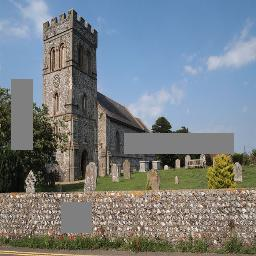
\includegraphics[width=.16\textwidth]{figures/teaser/000000120572_input_image.jpg}&
  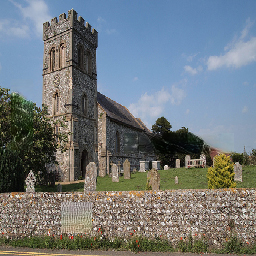
\includegraphics[width=.16\textwidth]{figures/teaser/output_mask17.jpg}&
  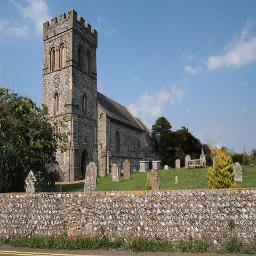
\includegraphics[width=.16\textwidth]{figures/teaser/000000120572_synthesized_image.jpg} &
    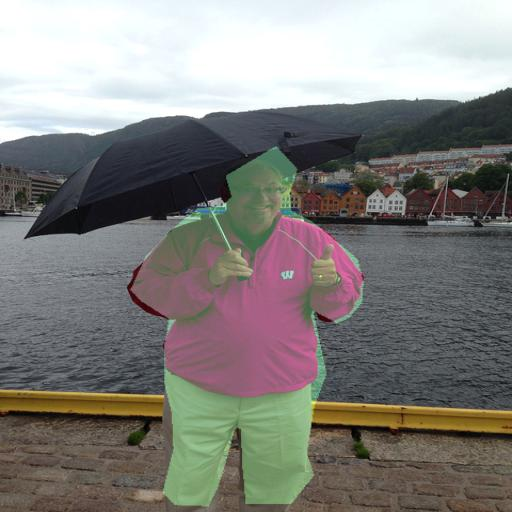
\includegraphics[width=.16\textwidth]{figures/teaser/input.jpg}&
  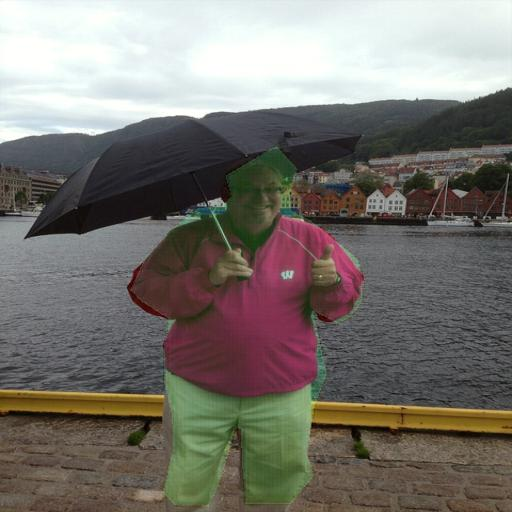
\includegraphics[width=.16\textwidth]{figures/teaser/dh.jpg}&
  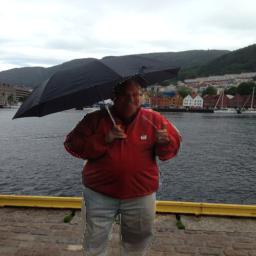
\includegraphics[width=.16\textwidth]{figures/teaser/ours.jpg} \\
  (a) Input  & (b) GLI~\cite{iizuka2017globally} & (c) Ours & (c) Input  & (d) DH~\cite{tsai2017deep} & (e) Ours  \\
\end{tabular}
\caption{An example of inpainting (top) and harmonzation (bottom) comparing with state-of-the-art methods. Zoom in for best viewing quality.}
\label{fig:teaser}
\vspace{-15pt}
\end{figure}

More recently, deep neural networks have shown excellent performance in various image completion tasks, such as texture synthesis and image completion. For inpainting, adversarial training becomes the de facto strategy to generate sharp details and natural looking results~\cite{pathak2016context,yeh2016semantic,li2017generative,yang2017high,iizuka2017globally}. Pathak et al.~\cite{pathak2016context} first proposes to train an encoder-decoder model for inpainting using both the reconstruction loss and adversarial loss. In~\cite{yeh2016semantic}, Yeh et al. uses a pre-trained model to find the most similar encoding of a corrupted image and uses the found encoding to synthesize what is missing. In~\cite{yang2017high}, Yang et al. proposes a multi-scale approach and optimizes the hole contents such that its neural feature extracted from a pre-trained CNN matches with the features of the surrounding context. The optimization scheme improves the inpainting quality and resolution at the cost of computational efficiency. In~\cite{iizuka2017globally}, Iizuka et al. proposes a deep generative model trained with global and local adversarial losses, and can achieve good inpainting performance for mid-size images and holes. However, it requires extensive training (two months as described in the paper), and the results often contain excessive artifacts and noise patterns. Another limitation of ~\cite{yang2017high} and ~\cite{iizuka2017globally} is that they are unable to handle perceptual discontinuity, making it necessary to resort to post-processing (e.g. Poisson blending).

In practice, we found that directly training a very deep generative network to synthesize high-frequency details is challenging due to optimization difficulty and unstable adversarial training. As a result, as the network becomes deeper, the inpainting quality may worsen. To overcome this difficulty, we discuss a new training scheme that guides and stabilizes the training of a very deep generative model, which, combining with carefully designed training losses, significantly reduces the artifacts and improves the quality of results. The main strategy, referred to as \textbf{B}lock-wise \textbf{P}rocedural \textbf{T}raining (\textbf{BPT}), progressively increases the number of residual blocks and the depth of the network. With BPT, we first train a cGAN-based \textbf{Generator Head} until converging, followed by adding additional residual blocks one at a time to refine and improve the results. This enables us to train a network deeper than~\cite{iizuka2017globally} and generates more realistic-looking details. We also observe that to reduce the noise level, it is essential to steadily reduce the weight of the adversarial loss given to the generator. We refer to this training scheme as \textbf{A}dversarial \textbf{L}oss \textbf{A}nnealing (\textbf{ALA}). Finally, we also propose several new losses specifically designed for inpainting: the \textbf{P}atch \textbf{P}erceptual \textbf{L}oss (\textbf{PPL}) and \textbf{M}ulti-\textbf{S}cale \textbf{P}atch \textbf{A}dversarial \textbf{L}oss (\textbf{MSPAL}). Experiments show that these losses work better than traditional losses used for inpainting, such as $\ell_2$ and the more general adversarial loss.

To evaluate the proposed approach, we conduct extensive experiments on a variety of datasets. Shown by qualitative and quantitative results, also by the user-study, our approach generates high-quality inpainting results and outperforms other state-of-the-art methods.  We also show that our framework, although being designed for inpainting, can be directly applied on general image translation tasks such as image harmonization and composition, and easily achieve results superior to other methods (Fig.~\ref{fig:teaser}). This enables us to train a multi-task model and use it for interactive guided inpainting, which is a very common and useful image editing scenario. We will describe it in detail in Sec.~\ref{exp:guided}.

In summary, in this paper we present:
\begin{enumerate}
\item A novel and effective framework that generates high-quality results for several image editing tasks like inpainting and harmonization. We also provide a thorough analysis and ablation study about the components in our framework.  
\item Extensive qualitative and quantitative evaluations on a variety of datasets, such as scenes, objects, and faces. We also conduct a user-study to make fair and rigorous comparisons with other state-of-the-art methods. 
\item Results of interactive guided inpainting as a novel and useful application of our approach. 
\end{enumerate}